%! Tex program = pdflatex
 
\documentclass[UTF8]{ctexart}
\CTEXsetup[format={\Large\bfseries}]{section}
\usepackage{amsmath}
\usepackage{ctex}
\usepackage{array}
\usepackage{ulem}
\usepackage{graphicx}
\usepackage{geometry}
\usepackage{multirow}
\usepackage{subfig}
\usepackage{float}
\usepackage{multicol}
\usepackage{multirow}
\usepackage{indentfirst}
\usepackage{makecell}
\usepackage{listings, xcolor}
\lstdefinestyle{lfonts}{
  basicstyle   = \footnotesize\ttfamily,
  stringstyle  = \color{purple},
  keywordstyle = \color{blue!60!black}\bfseries,
  commentstyle = \color{olive}\scshape,
}
\lstdefinestyle{lnumbers}{
  numbers     = left,
  numberstyle = \tiny,
  numbersep   = 1em,
  firstnumber = 1,
  stepnumber  = 1,
}
\lstdefinestyle{llayout}{
  breaklines       = true,
  tabsize          = 2,
  columns          = flexible,
}
\lstdefinestyle{lgeometry}{
  xleftmargin      = 20pt,
  xrightmargin     = 0pt,
  frame            = tb,
  framesep         = \fboxsep,
  framexleftmargin = 20pt,
}
\lstdefinestyle{lgeneral}{
  style = lfonts,
  style = lnumbers,
  style = llayout,
  style = lgeometry,
}
\lstdefinestyle{python}{
  language = {Python},
  style    = lgeneral,
}
\geometry{papersize={21cm,29.7cm}}
\geometry{left=2.54cm,right=2.54cm,top=3.18cm,bottom=3.18cm}
\usepackage{fancyhdr}
\pagestyle{fancy}
\lhead{\today}
\chead{}
\rhead{2020011075}
\lfoot{清华大学}
\cfoot{\thepage}
\rfoot{系统工程导论}
\renewcommand{\headrulewidth}{0.4pt}
\renewcommand{\headwidth}{\textwidth}
\renewcommand{\footrulewidth}{0pt}
\usepackage{bm}

\begin{document}

\begin{center}
  \textbf{\LARGE{系统工程导论作业五——主成分分析}}\\
\end{center}
\begin{center}
  \large{彭程 2020011075}
\end{center}


\noindent \textbf{\zihao{-4}{1.使用PCA和线性回归对附件的数据进行建模}}\\

\noindent \textbf{\zihao{-4}{1.1 算法思路}}

\noindent 1.样本数据规范化,消除单位影响。

$$
\bar{x}_{i}(t)=\frac{x_{i}(t)-e\left(x_{i}\right)}{\sqrt{\delta^{2}\left(x_{i}\right)}} ~~\forall i, t
$$

其中,  $e\left(x_{i}\right)=\frac{1}{N} \sum_{t=1}^{N} x_{i}(t)$  为样本均值, $ \delta^{2}\left(x_{i}\right)=\frac{1}{N-1} \sum_{t=1}^{N} \left(x_{i}(t)-e\left(x_{i}\right)\right)^{2} $ 为样本方差
$$
\bar{y}(t)=\frac{y(t)-e(y)}{\sqrt{\delta^{2}(y)}} ~~\forall t
$$
\noindent 2.根据阈值确定最优维度m

对归一化的协方差矩阵  $\Sigma =  \frac{1}{N-1} X X^{T}$  进行特征值分解。按照特征值从大到小选取特征向量, 直到相对逼近误差(末选取的特征值占特征值的比例)小于选取的阈值。\\

\noindent 3.求出降维后的矩阵。

将特征向量组成矩阵 $ Q_{m}=[q(1) q(2) \cdots q(m)] $,从而降维后的矩阵为$Z=Q_{m}^T X $。\\

\noindent 4.计算降维后的回归系数d,从而确定降维前的回归系数c,恢复得到归一化前的回归系数
$$
\begin{array}{c}
\hat{d}=\left(Z Z^{T}\right)^{-1} Z Y^{T} \\
\hat{\beta}=Q_{m} \hat{d}
\end{array}
$$

\noindent 5.进行显著性检验

对计算得到的回归系数进行显著性检验,注意其中n为降维之后的维度m:
$$
F=\frac{(N-n-1) E S S}{n R S S}
$$

\noindent 7.求取置信区间


给定显著性水平 $ \alpha $, 对某一  $\mathrm{x}_{0}$ , 相应的  $\mathrm{y}_{0} $ 将以 $ 1-\alpha$  的概率落在置信区间:
$$
\left(\hat{y}_{0}-Z_{\alpha / 2} S_{\delta}, \hat{y}_{0}+Z_{\alpha / 2} S_{\delta}\right)
$$

其中 $ Z_{\alpha / 2} $ 是标准正态分布上  $\alpha / 2 $ 百分位点的值, 剩余均方差  $S_{\delta}=\sqrt{\frac{R S S}{N-n-1}}$。\\

\noindent \textbf{\zihao{-4}{1.2 实验结果}}

\begin{figure}[H]
  \centering
  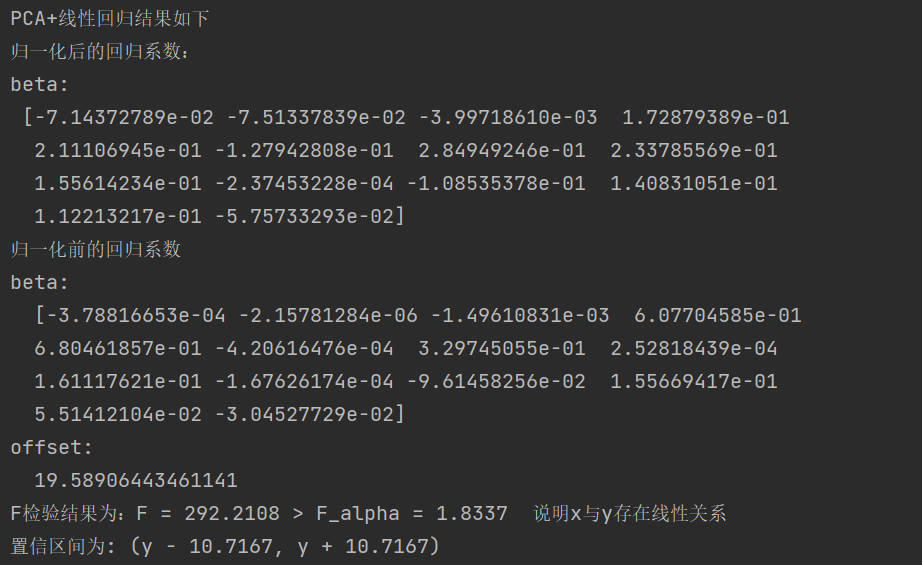
\includegraphics[scale=0.3]{PCA结果.jpg}
\end{figure}

\begin{figure}[H]
  \centering
  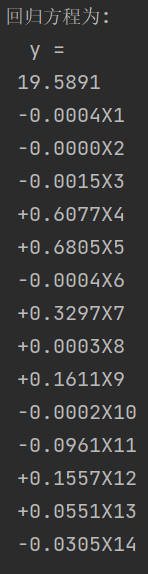
\includegraphics[scale=0.3]{PCA回归方程.jpg}
\end{figure}

\noindent 根据上述结果,回归方程为:

$\begin{aligned} y=19.5891-& 0.0004 X_1-0.0000 X_2-0.0015 X_3+0.6077 X_4+0.6805 X_5 \\ &-0.0004 X_6+0.3297 \times 7+0.0003 X_8+0.1611 X_9-0.0002 X_{10} \\ &-0.0961 X_{11}+0.1557 X_{12}+0.0551 X_{13}-0.0305 X_14 \end{aligned}$\\


\noindent $ \mathrm{F}$  检验: $F = 292.2108 > F_\alpha = 1.8337  $ , 因此  x, y  存在线性关系。\\

\noindent 置信区间:  $(y - 10.7167, y + 10.7167) $\\


\noindent \textbf{\zihao{-4}{1.3 协方差矩阵系数选取}}

在编程中协方差矩阵的分母为N - 1。 根据概统的知识, 当分母为N - 1 时可以得到样本协方差的无偏估计。 但其实在本次作业中, 使用N和N - 1对实验结果并没有影响,因为我们是通过相对误差上限来选出最大的r 个特征向量,与前面的这个系数没有关系。\\\\\\\\

\noindent \textbf{\zihao{-4}{2.使用病态线性回归对附件的数据进行建模}}\\

\noindent \textbf{\zihao{-4}{2.1 算法思路}}

和上次作业中的思路完全相同,此处仅展示结果。

\noindent \textbf{\zihao{-4}{2.1 实验结果}}

\begin{figure}[H]
  \centering
  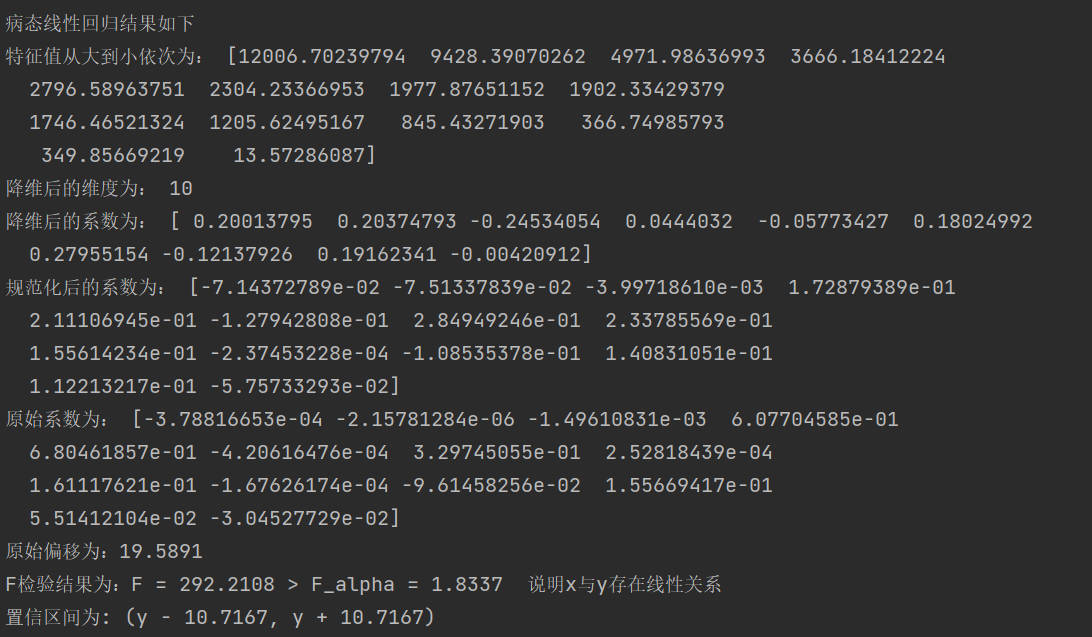
\includegraphics[scale=0.3]{病态结果.jpg}
\end{figure}

\begin{figure}[H]
  \centering
  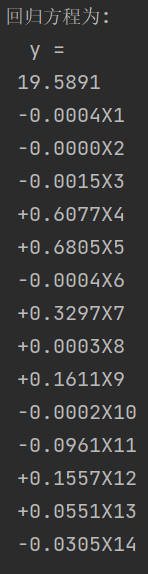
\includegraphics[scale=0.3]{PCA回归方程.jpg}
\end{figure}

可以看到病态线性回归结果和PCA主成分分析结果完全相同,说明两者的操作是等价的。\\


\noindent \textbf{\zihao{-4}{3.附代码}}\\



\begin{lstlisting}[style = python]
  import numpy as np
  from scipy import stats
  import pandas as pd
  
  
  def pca_compress(data, rerr):
      """
      输入:
          -data:输入的原始数据 N*(n+1)
          -rerr:相对误差界限
      输出:
          -pcs:主成分
          -cprs_data:压缩后的数据
          -cprs_c:压缩时的常数
      功能:实现主成分分析
      """
  
      # data
      x = data[:, 0: -1].T  # 规模 n*N
      n, N = x.shape
  
      # 规范化:
      x_mean = np.mean(x, axis=1, keepdims=True)
      x_std = np.std(x, axis=1, keepdims=True, ddof=1)
      x_norm = (x - x_mean) / x_std
  
      # 存恢复参数
      cprs_c = {}
      cprs_c["x_mean"] = x_mean
      cprs_c["x_std"] = x_std
  
      # 主成分分析
      eigenvalue, eigenvector = np.linalg.eig(np.dot(x_norm, x_norm.T))
      eigen_index = np.argsort(-eigenvalue)  # 返回排序的下标,从大到小
      eigen_sum = np.sum(eigenvalue)
      eigen_error = eigen_sum
      for m in range(0, n):
          eigen_error = 0
          for i in range(0, m):
              eigen_error += eigenvalue[eigen_index[n - 1 - i]]
          eigen_error = eigen_error / eigen_sum
          if eigen_error > rerr:
              break
      m = n - m + 1  # 前m项保留
      pcs = eigenvector[:, eigen_index[0: m]]
      cprs_data = x_norm.T.dot(pcs)
      # print(pcs.shape)
      # print(cprs_data.shape)
  
      return pcs, cprs_data, cprs_c
  
  
  def pca_reconstruct(pcs, cprs_data, cprs_c):
      """
      输入:
          -pcs:主成分(14*10)
          -cprs_data:压缩后的数据(3114*10)
          -cprs_c:压缩时的常数
      输出:
          -recon_data: 恢复的数据 N*n  (3114*14)
      功能:实现数据恢复
      """
      recon_data_norm = cprs_data.dot(pcs.T)
      recon_data = recon_data_norm * cprs_c["x_std"].T + cprs_c["x_mean"].T
      return recon_data
  
  
  def pca_linear_regression(data, alpha=0.05, error=0.05):
      """
      输入:
          -pcs:主成分
          -cprs_data:压缩后的数据
          -cprs_c:压缩时的常数
      输出:
          -recon_data: 恢复的数据
      功能:实现完整主成分分析+线性回归
      """
  
      x = data[:, 0: 14].T
      y = data[:, 14]
      y_mean = np.mean(y.T)
      y_std = np.std(y, ddof=1)
      y_norm = (y - y_mean) / y_std
      n = x.shape[0]
      N = x.shape[1]
  
      # pca
      # print("初始数据\n", data)
      pcs, cprs_data, cprs_c = pca_compress(data, error)
      # print("压缩数据\n", cprs_data)
      recon_data = pca_reconstruct(pcs, cprs_data, cprs_c)
      # print("恢复数据\n", recon_data)
      Z = cprs_data.T
  
      # regression coefficient after normalization
      d = np.linalg.inv(np.dot(Z, Z.T)).dot(Z.dot(y_norm.T))  # 最小二乘
      beta = np.dot(pcs, d)
      print("归一化后的回归系数:")
      print("beta: \n", beta)
  
      # 恢复得到归一化前的回归系数beta
      beta = beta / cprs_c["x_std"].reshape(-1) * y_std
      offset = y_mean - np.sum(beta.reshape(-1,1)  * cprs_c["x_mean"].reshape(-1, 1))
  
  
      print("归一化前的回归系数")
      print("beta:\n ", beta)
      print("offset:\n ", offset)
  
      # F检验
      r = pcs.shape[1]
      y_estimate = np.dot(beta.T, x) + offset
      ess = np.dot((y_estimate - y_mean).T, (y_estimate - y_mean))
      rss = np.dot((y - y_estimate).T, (y - y_estimate))
      F = ((N - r - 1) * ess) / (r * rss)
      F_alpha = stats.f.isf(alpha, r, N - r - 1)
      if F > F_alpha:
          print("F检验结果为:F = {:.4f} > F_alpha = {:.4f}".format(F, F_alpha), " 说明x与y存在线性关系")
      elif F <= F_alpha:
          print("F检验结果为:")
          print("F-value = {:.4f} <= F_alpha = {:.4f}".format(F, F_alpha))
          print("x与y不存在线性关系")
          return 0
  
      # 打印置信区间
      S_delta = np.sqrt(rss / (N - r - 1))
      Z_alpha_div2 = stats.norm.isf(alpha / 2, 0, 1)
      interval = Z_alpha_div2 * S_delta
      print("置信区间为: (y - {:.4f}, y + {:.4f})".format(interval, interval))
  
      # 打印回归方程
      equation = "y =\n %.4f\n" % offset
      for i in range(n):
          equation += " %+.4fX%d\n" % (beta[i], i + 1)
      print("回归方程为:\n ", equation)
  
      return beta, offset
  
  
  def morbid_linear_regression(Y, X, alpha=0.05, error=0.01):
      """
      输入:n×N的矩阵X,1×N的矩阵Y
      输出:N×1的回归系数theta
      功能:实现Y=c^T*X+b的多元线性回归,自适应病态线性回归
      """
      n, N = X.shape
  
      # 数据规范化
      x_mean = np.mean(X, axis=1, keepdims=True)
      delta_x = np.sqrt(
          np.sum(np.multiply(X - np.mean(X, axis=1, keepdims=True), X - np.mean(X, axis=1, keepdims=True)), axis=1,
                 keepdims=True) / (N - 1))
      X_normal = np.divide(X - x_mean, delta_x)
      y_mean = np.mean(Y)
      delta_y = np.sqrt(np.sum(np.multiply(Y - y_mean, Y - y_mean)) / (N - 1))
      Y_normal = (Y - y_mean) / delta_y
  
      # 根据阈值确定最优维度m
      eigenvalue, eigenvector = np.linalg.eig(np.dot(X_normal, X_normal.T))
      eigen_index = np.argsort(-eigenvalue)  # 返回排序的下标
      eigen_sum = np.sum(eigenvalue)
      for m in range(0, n):
          eigen_error = 0
          for i in range(0, m):
              eigen_error += eigenvalue[eigen_index[n - 1 - i]]
          eigen_error = eigen_error / eigen_sum
          if eigen_error > error:
              break
      m = n - m + 1  # 则前m项是要保留的
  
      # 计算降维后的回归系数d,从而确定降维前的回归系数c_n,恢复得到归一化前的回归系数c
      Q = eigenvector[:, eigen_index[0: m]]
      Z = Q.T.dot(X_normal)
      d = np.linalg.inv(Z.dot(Z.T)).dot(Z.dot(Y_normal.T))
      c_n = Q.dot(d)
      c_n=c_n.reshape(-1)
      c = (c_n.T / np.squeeze(delta_x) * delta_y).T
      c=c.reshape(-1)
      b = y_mean - np.sum(c * np.squeeze(x_mean))
      print("特征值从大到小依次为:", eigenvalue[eigen_index[:]])
      print("降维后的维度为:", m)
      print("降维后的系数为:", d)
      print("规范化后的系数为:", c_n)
      print("原始系数为:", c)
      print("原始偏移为:{:.4f}".format(b))
  
      # F检验操作
      Y_estimate = np.dot(c.T, X) + b
      ESS = np.dot((Y_estimate - y_mean), (Y_estimate - y_mean).T)
      RSS = np.dot((Y - Y_estimate), (Y - Y_estimate).T)
      F = ((N - m - 1) * ESS) / (m * RSS)  # ESS自由度为(N-m-1),RSS自由度为m
      F_alpha = stats.f.isf(alpha, m, N - m - 1)
  
      if F > F_alpha:
          print("F检验结果为:F = {:.4f} > F_alpha = {:.4f}".format(F, F_alpha), " 说明x与y存在线性关系")
      elif F <= F_alpha:
          print("F检验结果为:")
          print("F-value = {:.4f} <= F_alpha = {:.4f}".format(F, F_alpha))
          print("x与y不存在线性关系")
          return 0
  
      # 置信区间
      S_delta = np.sqrt(RSS / (N - m - 1))
      Z_alpha_div2 = stats.norm.isf(alpha / 2, 0, 1)
      interval = Z_alpha_div2 * S_delta
      print("置信区间为: (y - {:.4f}, y + {:.4f})".format(interval, interval))
  
      # 打印回归方程
      equation = "y = %.4f" % b
      for i in range(n):
          equation += " + %.4fX%d" % (c[i], i + 1)
      print("回归方程为: ", equation)
  
      return
  
  
  if __name__ == '__main__':
      raw_data = pd.read_excel('counties.xlsx', usecols='C:Q')
      data = np.array(raw_data)
      x = data[:, 0: 14].T
      y = data[:, 14]
  
      # PCA+线性回归
      print("PCA+线性回归结果如下")
      pca_linear_regression(data, alpha=0.05, error=0.05)
      # 直接病态线性回归
      print("病态线性回归结果如下")
      morbid_linear_regression(y, x, alpha=0.05, error=0.05)
  
\end{lstlisting}      


\end{document}